
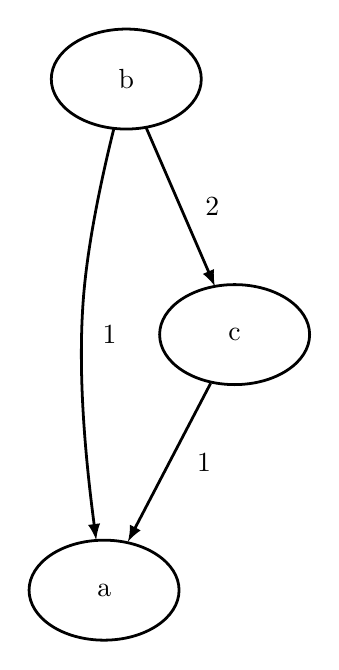
\begin{tikzpicture}[>=latex,line join=bevel,]
  \pgfsetlinewidth{1bp}
%%
\pgfsetcolor{black}
  % Edge: b -> a
  \draw [->] (30.497bp,184.04bp) .. controls (26.84bp,169.34bp) and (21.976bp,147.44bp)  .. (20.0bp,128.0bp) .. controls (17.165bp,100.11bp) and (19.937bp,68.092bp)  .. (24.168bp,36.025bp);
  \definecolor{strokecol}{rgb}{0.0,0.0,0.0};
  \pgfsetstrokecolor{strokecol}
  \draw (29.0bp,110.0bp) node {1};
  % Edge: c -> a
  \draw [->] (65.379bp,92.493bp) .. controls (58.357bp,79.045bp) and (48.322bp,59.83bp)  .. (35.566bp,35.403bp);
  \draw (63.0bp,64.0bp) node {1};
  % Edge: b -> c
  \draw [->] (42.153bp,184.49bp) .. controls (47.926bp,171.17bp) and (56.15bp,152.19bp)  .. (66.892bp,127.4bp);
  \draw (66.0bp,156.0bp) node {2};
  % Node: a
\begin{scope}
  \definecolor{strokecol}{rgb}{0.0,0.0,0.0};
  \pgfsetstrokecolor{strokecol}
  \draw (27.0bp,18.0bp) ellipse (27.0bp and 18.0bp);
  \draw (27.0bp,18.0bp) node {a};
\end{scope}
  % Node: c
\begin{scope}
  \definecolor{strokecol}{rgb}{0.0,0.0,0.0};
  \pgfsetstrokecolor{strokecol}
  \draw (74.0bp,110.0bp) ellipse (27.0bp and 18.0bp);
  \draw (74.0bp,110.0bp) node {c};
\end{scope}
  % Node: b
\begin{scope}
  \definecolor{strokecol}{rgb}{0.0,0.0,0.0};
  \pgfsetstrokecolor{strokecol}
  \draw (35.0bp,202.0bp) ellipse (27.0bp and 18.0bp);
  \draw (35.0bp,202.0bp) node {b};
\end{scope}
%
\end{tikzpicture}

